\chapter{Aufnahme von Koordinatenpunkte}
\section{Problem}
Wenn ein Koordinatenpunkt aufgenommen werden will, gibt es mehrere Probleme auf die man stößt.

Zum einen kann nicht gleichzeitig die X und Y Komponente der Koordinate bestimmt werden. Dies muss nacheinander folgen.
Grund hierfür ist dem Aufbau des Touchscreens geschuldet.

Bei der Inbetriebnahme wird sich noch ein weiteres Problem ergeben.
Falls der Touchscreen nicht betätigt wird, gibt der Mikrocontroller trotzdem Werte aus.
Dabei handelt es sich um Werte die keinen Sinn ergeben und die Steuerung der Maus z.B. bei einer Ruhephase stören würden.

Bei einer Messreihe kann es vereinzelt zu einem Wertesprung kommen. 
Dieses Problem ist der Messunsicherheit des Systems geschuldet. 
Diese Sprünge gilt es aus der Messreihe heraus zu filter und zu glätten.

\section{Lösungsansatz}
Um das Problem, bei einer nicht Betätigung des Touchscreens, zu lösen, soll vor einer Aufnahme von Koordinatenwerte geprüft werden, ob der Touchscreen betätigt wird.
Ist dies der Fall so soll die Messung durchgeführt werden.

Um eine Koordinatenkomponente zu bestimmen, benötigt man drei Anschlüsse des Touchscreens.
Zwei davon sind in der Richtung die man messen möchte und der dritte Anschluss ist einer der beiden übrigen Anschlüsse.
Mit diesem wird der Spannungsteiler auf gespannt um den Wert der Koordinate zu bestimmen.

In den \cref{fig:xylesen} auf \cref{fig:xylesen} wird dieser Lösungsansatz veranschaulicht.
Bei dem Lesen der x-Komponente \cref{fig:xlesen} wird der Pin \verb$X_Le$ (steht für X-Links) auf eine Spannung von \SI{5}{V} gesetzt.
Der Pin \verb$X_Ri$ (steht für X-Rechts) wird auf \SI{0}{V} gezogen.
Der Pin  \verb$Y_Up$ (steht für Y-Oben) wird auf den Modus \verb$Hi Z$ (Hohe Eingangsimpedanz) gesetzt. In diesem Modus fällt der Widerstand in die y-Richtung so klein aus, das er vernachlässigbar gering ist.
Um die y-Komponente zu lesen wird das wie in \cref{fig:ylesen} auf \cpageref{fig:ylesen} der Pin \verb$Y_Up$ auf \SI{5}{V} gesetzt und der Pin \verb$Y_Lo$ (steht für Y-Unten) auf \SI{0}{V} gesetzt.
Hier wird der \verb$Hi Z$ Modus auf den Pin \verb$X_Le$ gesetzt.

Um nun noch eine Messunsicherheiten aus zu filtern sollen, bei der Messung einer Koordinatenkomponente, mehrere Messpunkte aufgenommen werden.
Diese werden anschließend über ein Filter-Funktion ausgewertet.
Der Wert der bei der Auswertung als Ergebnis herauskommt, wird als gemessene Koordinatenkomponente ausgegeben.
Das Schaltbild hierzu ist in \cref{fig:schaltbild} zu sehen.

\begin{figure}[ht!]
    \begin{subfigure}{0.49\textwidth}
        \centering
        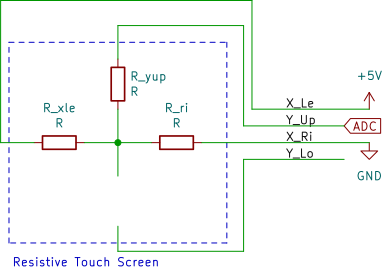
\includegraphics[width=\textwidth]{fig/xlesen.png}
        \caption{in x-Richtung}
        \label{fig:xlesen}
    \end{subfigure}
    \hfill
    \begin{subfigure}{0.49\textwidth}
        \centering
        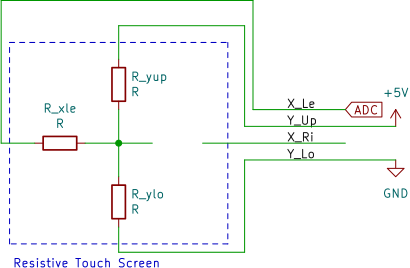
\includegraphics[width=\textwidth]{fig/ylesen.png}
        \caption{in y-Richtung}
        \label{fig:ylesen}
    \end{subfigure}
    \caption{Schaltbild für das Messen der Koordinatenpunkte}
    \label{fig:xylesen}
\end{figure}
\begin{figure}[ht!]
    \centering
    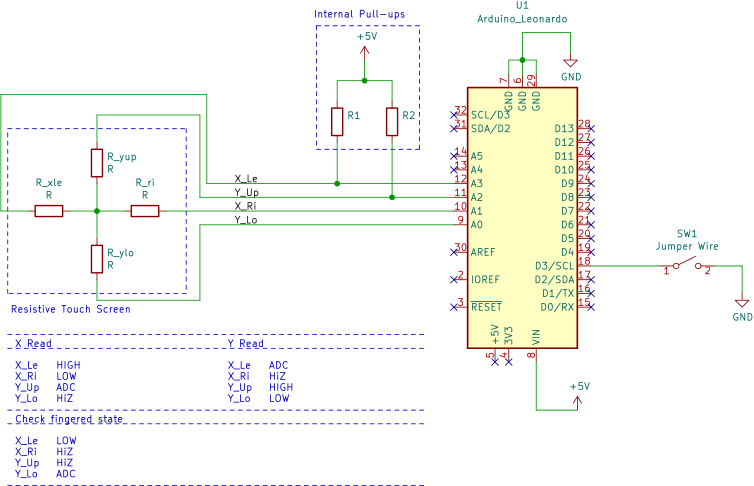
\includegraphics[width=\linewidth]{fig/schaltbild.png}
    \caption{Schaltbild des Projekts}
    \label{fig:schaltbild}
\end{figure}
Die einzelne Lösungsansätze werden in der Arduino-Umgebung umgesetzt.
Der Programmablauf ist in \cref{fig:flowchart} als Flow-Chart dargestellt.

\begin{figure}
    \centering
    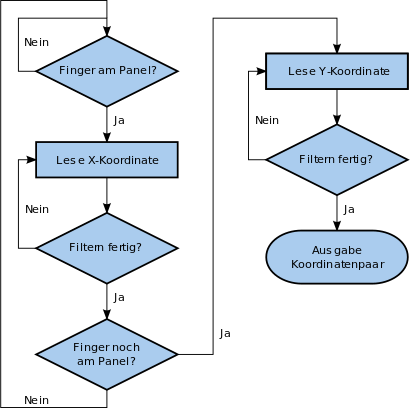
\includegraphics[scale=0.45]{fig/flow_chart.png}
    \caption{Darstellung des Programmablaufs}
    \label{fig:flowchart}
\end{figure}
